% CS3103 PBL report -- AI trading indicator for JPM
% Build: latexmk -pdf main.tex   (or upload the report/ folder to Overleaf, compiler pdfLaTeX)
\documentclass[11pt,a4paper]{article}

\usepackage[T1]{fontenc}
\usepackage[utf8]{inputenc}
\usepackage[a4paper,margin=2cm,columnsep=0.7cm]{geometry}
\usepackage{amsmath,amssymb}
\usepackage{graphicx}
\usepackage{booktabs,tabularx}
\usepackage{float}
\usepackage{caption,subcaption}
\usepackage{enumitem}
\usepackage{algorithm}
\usepackage{algpseudocode}
\usepackage{tikz}
\usetikzlibrary{positioning,arrows.meta,calc}
\usepackage{microtype}
\usepackage[hidelinks]{hyperref}
\setlength{\emergencystretch}{2em}

\graphicspath{{figures/}}
\captionsetup{font=small,labelfont=bf}
\setlist{itemsep=1pt,topsep=2pt,leftmargin=1.2em}

\begin{document}

% ---------------------------------------------------------------- title page
\begin{titlepage}
\centering
\vspace*{2cm}
{\large CS3103 -- Project-Based Learning (Machine Learning)\par}
\vspace{1.5cm}
{\LARGE\bfseries An AI Trading Indicator for\\[4pt] JPMorgan Chase (JPM)\par}
\vspace{1.5cm}
{\large Project Report\par}
\vspace{2cm}
\begin{tabular}{ll}
Submitted by & Tanishq Sangwan (2401AI42) \\
E-mail & tanishq\_2401ai42@iitp.ac.in \\
Instructor & Dr. Rishav Singh \\
Department & Computer Science and Engineering \\
Institute & Indian Institute of Technology Patna \\
Date & November 2026 \\
\end{tabular}
\vfill

\includegraphics[width=3cm]{iitp-logo.png}
\vspace*{1cm}
\end{titlepage}

% ---------------------------------------------------------------- contents (short)
\setcounter{page}{1}
\setcounter{tocdepth}{1}
\twocolumn[{\small\tableofcontents}\vspace{1em}]

% ================================================================
\section{Introduction}
Intraday stock prices move in small, noisy steps, and most ``buy/sell'' signals a new trader sees are never checked on
data they were not built on. The efficient-market view \cite{fama1970} says past prices should tell us little about the
next price change. On the other hand, intraday \emph{volatility} is known to follow strong patterns
\cite{andersen1997}, and order flow explains a lot of short-term moves \cite{cont2014}.

We picked JPMorgan Chase (JPM). It is the largest US bank and it moves closely with its sector: 5-min returns have
correlation 0.85 with the sector ETF XLF and 0.80 with Bank of America (Fig.~\ref{fig:eda}). So market, peer-bank and
news data should carry some information about the next few minutes.

\textbf{Problem.} Let $C_t$ be the JPM close of the 5-min candle ending at $t$. Using only data available up to $t$,
predict the class of the 10-min log return
\begin{equation}
  r_t = 10^4 \ln\frac{C_{t+2}}{C_t},
  \ y_t = \begin{cases} \text{Up} & r_t > \tau \\ \text{Down} & r_t < -\tau \\ \text{Flat} & \text{else} \end{cases}
  \label{eq:label}
\end{equation}
with $\tau = 5.53$\,bps, the 33rd percentile of $|r_t|$ on 2016--21, so the three classes are roughly equal. We also
predict how active the market will be, the chance of a big move, and a price range for the rest of the day.

\textbf{What we did.}
\begin{itemize}
  \item A causal feature pipeline (103 features) with leakage tests and a shuffled-label placebo check.
  \item A 3-class call that beats simple rules out of sample (40.7\,\% vs 35.8\,\%), plus activity, big-move
        (AUC 0.785) and price-band outputs.
  \item A negative result: ten model families could not predict plain direction.
  \item A replay dashboard that grades every call.
\end{itemize}
Scope: one stock, regular hours (09:30--16:00 ET), Jan 2016 to Nov 2026. The tool informs a person; it does not trade.

% ================================================================
\section{Related Work}
Lo and MacKinlay \cite{lo1988} rejected the pure random walk for weekly returns, and Brock et al.\ \cite{brock1992} found simple moving-average rules had some predictive power on the Dow before costs,
but such gains mostly disappear after costs and multiple-testing corrections \cite{bailey2014}. Gu, Kelly and Xiu
\cite{gu2020} showed trees and neural nets beat linear models for monthly returns, and Krauss et al.\
\cite{krauss2017} and Fischer and Krauss \cite{fischer2018} got daily S\&P~500 direction accuracy only a little above
50\,\%. Gradient boosting (XGBoost \cite{chen2016}, LightGBM \cite{ke2017}, CatBoost \cite{prokhorenkova2018}) is still
the strong default for tabular data.

Volatility is persistent and U-shaped over the day \cite{andersen1997,bollerslev1986}, which is why the \emph{size} of
a move is easier to forecast than its sign. Without trade data, buy/sell volume can be estimated with the tick rule
\cite{lee1991} or bulk volume classification \cite{easley2012}. Tetlock \cite{tetlock2007} showed negative media tone predicts downward pressure on prices; tone can be scored with
VADER \cite{hutto2014} or the finance-tuned FinBERT \cite{araci2019}. For uncertainty we follow Guo et al.\ \cite{guo2017} (calibration error) and conformalized
quantile regression \cite{romano2019}. L\'opez de Prado \cite{lopezdeprado2018} warns against random splits and
repeated back-testing, so we use walk-forward validation and a single final test.

Gaps we noticed: most papers report only direction on daily data, many intraday studies leak future data (e.g.\ news
rounded to the day), and calibration or band coverage is rarely checked.

% ================================================================
\section{Data}
One-minute OHLCV bars (with trade count and VWAP) from the Alpaca API, SIP feed (all US exchanges), for JPM, SPY
(market), XLF (sector) and five peer banks: BAC, C, WFC, GS, MS. Table~\ref{tab:data} gives the counts up to the end of 2024. Events: Alpaca news (publication time), earnings dates, FOMC statement times
and SEC filings (8-K, Form~4, 13D/G, 10-Q/10-K, by acceptance time).

\begin{table}[t]
\centering\small
\caption{1-min bars up to 31 Dec 2024 (regular + extended hours).}
\label{tab:data}
\begin{tabular}{@{}l l r@{}}
\toprule
Ticker & Role & Bars \\
\midrule
JPM & target & 1,037,473 \\
SPY & market ETF & 1,774,344 \\
XLF & sector ETF & 1,094,874 \\
BAC, C, WFC & peers & 1.04--1.29\,M each \\
GS, MS & peers & 0.94--0.95\,M each \\
\bottomrule
\end{tabular}
\end{table}

\textbf{Preprocessing.}
\begin{enumerate}
  \item Keep regular hours of complete sessions (NYSE calendar) and resample to 5-min candles (78 a day), aligned
        across tickers. 2016--24 gives \textbf{173,376} rows; 2025 onward is held back for testing.
  \item A feature at candle $t$ only uses bars closed at or before $t$ and news/filings published at or before $t$.
        Daily quantities come from the previous session.
  \item The last two candles of a day have no label (76 labelled per day).
  \item Missing values are left to LightGBM; for logistic regression we use median imputation and scaling.
\end{enumerate}

\textbf{EDA.} Fig.~\ref{fig:eda} shows the two things that shaped the model. 5-min moves are about three times bigger
in the first half hour than at midday, so time of day has to be a feature. And JPM moves with the sector (0.85 with
XLF, 0.66 with SPY). On the test period the classes are 33.1\,\% Down, 32.8\,\% Flat, 34.1\,\% Up.

\begin{figure*}[t]
  \centering
  \begin{subfigure}[b]{0.48\textwidth}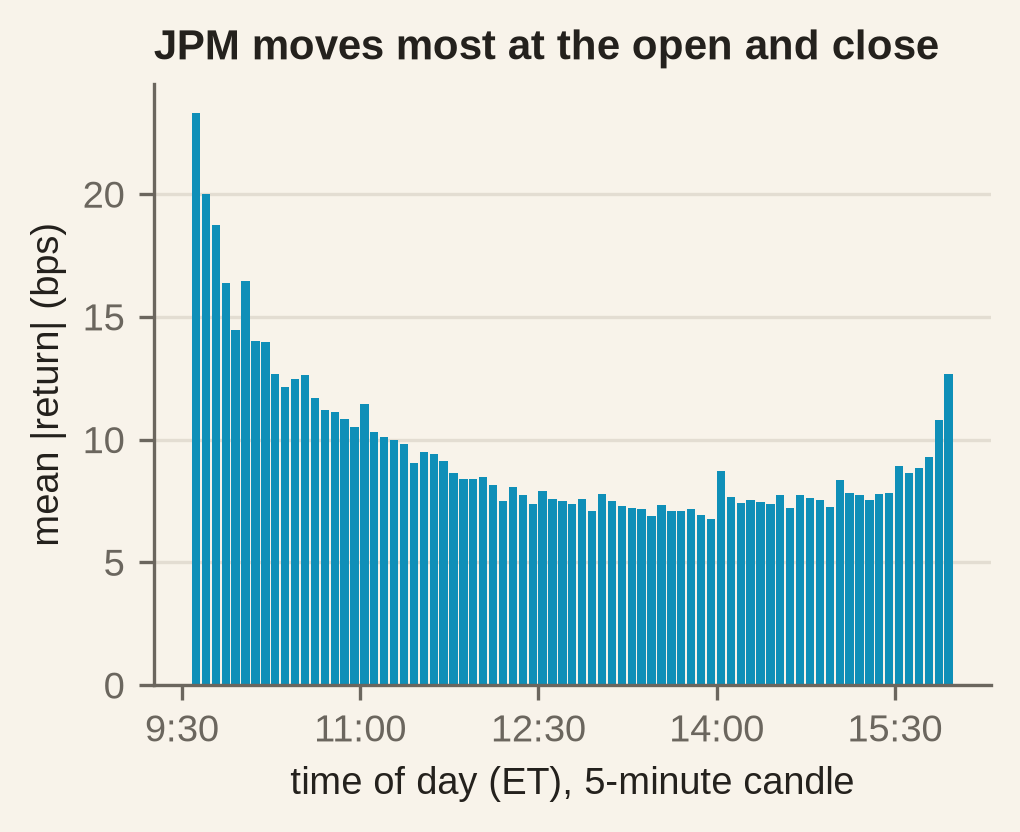
\includegraphics[width=\linewidth]{fig_eda_intraday.png}\caption{Mean $|$5-min move$|$ by time of day.}\end{subfigure}\hfill
  \begin{subfigure}[b]{0.40\textwidth}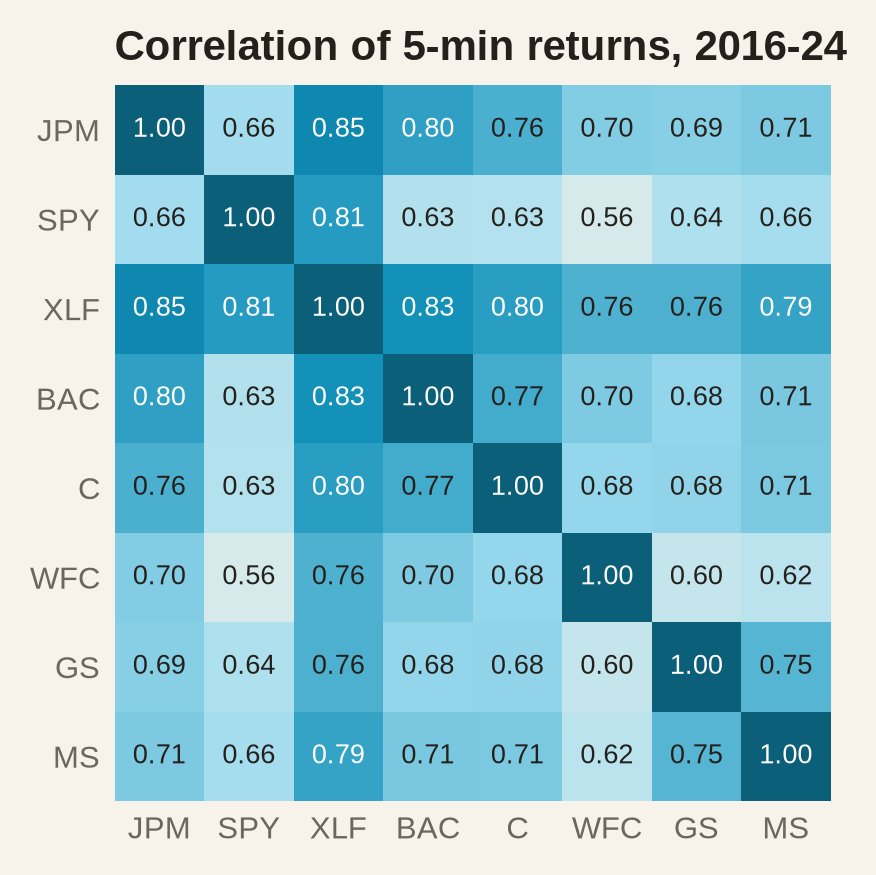
\includegraphics[width=\linewidth]{fig_eda_corr.png}\caption{Return correlations.}\end{subfigure}
  \caption{EDA on JPM 5-min returns, 2016--24.}
  \label{fig:eda}
\end{figure*}

% ================================================================
\section{Method}

\subsection{Features}
103 features in 7 families (Table~\ref{tab:feat}). Order-flow imbalance is approximated from bars in three ways: tick
rule \cite{lee1991}, close-location value $\frac{(C-L)-(H-C)}{H-L}$, and bulk volume classification
\cite{easley2012}. News tone is the VADER score \cite{hutto2014} of headline + summary, plus keyword flags (upgrade,
downgrade, price target, legal, earnings, dividend).

\begin{table}[t]
\centering\small
\caption{Feature families.}
\label{tab:feat}
\begin{tabularx}{\columnwidth}{@{}l c X@{}}
\toprule
Family & \# & Examples \\
\midrule
Volatility \& range & 10 & realised vol (1 h, 1 d, 5 d), Bollinger width \\
Market \& peers & 17 & SPY, XLF, peer returns; JPM vs peers \\
Volume \& order flow & 19 & imbalance (tick, CLV, BVC); trade size \\
Momentum & 17 & 5--120 min returns, RSI, MACD, VWAP gap \\
News \& events & 32 & news count/tone; time since earnings, FOMC \\
Day range & 5 & distance to today's/yesterday's high, low \\
Time & 3 & candle number, candles left, weekday \\
\bottomrule
\end{tabularx}
\end{table}

\subsection{Models}
Fig.~\ref{fig:arch} shows the system. One feature row per candle feeds the direction, activity and big-move models; a
separate 1-min model gives the next-minute call and the rest-of-day bands. Support/resistance lines (previous day
high/low/close, pivots, opening range, swing points) are plain rules, only drawn on the chart.

The direction model is LightGBM \cite{ke2017}: per class $k$ an ensemble of trees
$F_k(\mathbf{x}) = \sum_m \eta f_{k,m}(\mathbf{x})$, turned into probabilities by a softmax and trained on multi-class
log-loss. For the price bands, LightGBM quantile regression predicts 7 quantiles of the return to the close (pinball
loss), and conformalized quantile regression \cite{romano2019} widens it: with scores
$s_i = \max\{\hat y_{\text{lo}}(x_i) - y_i,\ y_i - \hat y_{\text{hi}}(x_i)\}$ on a calibration set and $E$ their
$\lceil(1-\alpha)(n+1)\rceil/n$ quantile, the band is $[\hat y_{\text{lo}} - E,\ \hat y_{\text{hi}} + E]$, with
coverage close to $1-\alpha$.

\begin{figure}[t]
\centering
\resizebox{\columnwidth}{!}{%
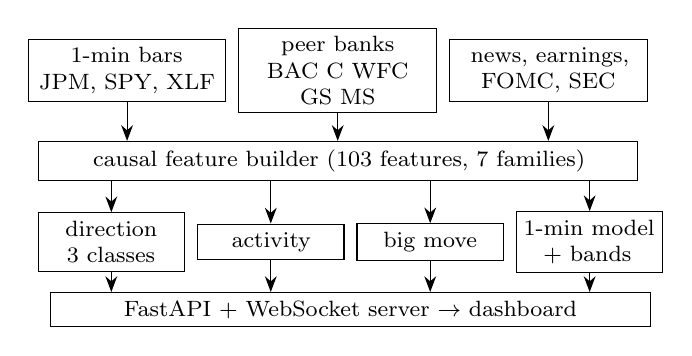
\begin{tikzpicture}[font=\footnotesize,
  box/.style={draw,align=center,inner sep=3pt,text width=#1},
  box/.default=2.3cm,
  arr/.style={-{Stealth[length=2mm]}},
  node distance=0.35cm and 0.15cm]
  \node[box] (m) {1-min bars\\JPM, SPY, XLF};
  \node[box,right=of m] (p) {peer banks\\BAC C WFC GS MS};
  \node[box,right=of p] (e) {news, earnings,\\FOMC, SEC};
  \node[box=7.4cm,below=of p] (f) {causal feature builder (103 features, 7 families)};
  \foreach \n in {m,p,e} \draw[arr] (\n.south) -- (\n.south |- f.north);
  \node[box=1.65cm,below=0.4cm of f.south west,anchor=north west] (d) {direction\\3 classes};
  \node[box=1.65cm,right=of d] (a) {activity};
  \node[box=1.65cm,right=of a] (b) {big move};
  \node[box=1.65cm,right=of b] (q) {1-min model\\+ bands};
  \foreach \n in {d,a,b,q} \draw[arr] (f.south -| \n.north) -- (\n.north);
  \node[box=7.4cm,below=0.4cm of $(a.south)!0.5!(b.south)$] (s) {FastAPI + WebSocket server $\to$ dashboard};
  \foreach \n in {d,a,b,q} \draw[arr] (\n.south) -- (\n.south |- s.north);
\end{tikzpicture}}
\caption{System overview.}
\label{fig:arch}
\end{figure}

\subsection{Training and validation}
Algorithm~\ref{alg:wf}. Each year is predicted by a model that has only seen earlier years. We did not tune much; the
settings in Table~\ref{tab:setup} were picked to be conservative (big leaves, strong regularisation) because the
signal is weak and overfitting was the main worry.

\begin{table}[t]
\centering\small
\caption{Setup and hyper-parameters.}
\label{tab:setup}
\begin{tabularx}{\columnwidth}{@{}l X@{}}
\toprule
Item & Setting \\
\midrule
Split & walk-forward; validation 2022--24 (56,843 candles); test 2025-01-02 .. 2026-10-27 (34,538); unseen 2026-10-28 .. 11-13 (988) \\
Horizon & 10 min (2 candles), $\tau=5.53$\,bps; big move $|r|>19.7$\,bps \\
LightGBM & 400 trees, lr 0.03, 15 leaves, $\geq$300 per leaf, subsample 0.7, L2 10 \\
Quantile GBM & 120 trees, lr 0.05, 15 leaves, $\geq$300 per leaf \\
LogReg & median impute, standardise, L2, $C=0.05$ \\
Cost & 2\,bps round trip \\
\bottomrule
\end{tabularx}
\end{table}

\begin{algorithm}[t]
\small
\caption{Walk-forward training of the 3-class call}
\label{alg:wf}
\begin{algorithmic}[1]
\State $\tau \gets$ 33rd pct of $|r|$ on 2016--21; $y$ by Eq.~\eqref{eq:label}
\State placebo: fit on shuffled $y$; \textbf{stop} if acc $>$ majority $+1.5$ pp
\For{$Y = 2022, \dots, 2026$}
  \State fit LightGBM and LogReg on all candles before $Y$
  \State predict $\hat P(\text{Up},\text{Flat},\text{Down})$ for year $Y$
\EndFor
\State pick the model with lowest log-loss on 2022--24
\State report it once on 2025-01-02 \dots 2026-10-27
\State refit on all data up to 2026-10-27, save, serve
\end{algorithmic}
\end{algorithm}

\textbf{Leakage checks.} (1) Features computed on truncated data must equal those on full data (max difference 0).
(2) Deleting news published after a bar must not change that bar's features. (3) Replay sweep: 365,352 checks of
what the dashboard shows vs what was known at the time, 0 leaks. (4) Training stops if any single feature has
$|\text{IC}| > 0.06$ with the label, or if the placebo predicts.

\textbf{Metrics.} For $N$ candles with true class $y_i$ and predicted probabilities $\hat p_{i,k}$:
\begin{align}
  \text{Acc} &= \tfrac{1}{N}\textstyle\sum_i \mathbb{1}[\arg\max_k \hat p_{i,k} = y_i],\\
  \text{LL} &= -\tfrac{1}{N}\textstyle\sum_i \ln \hat p_{i,y_i},\\
  \text{ECE} &= \tfrac{1}{3}\textstyle\sum_{k}\sum_{b=1}^{10} \tfrac{|B_{k,b}|}{N}\big|\bar y_{k,b} - \bar p_{k,b}\big|,
\end{align}
where $B_{k,b}$ is the $b$-th probability bin for class $k$ \cite{guo2017}. The big-move warning is scored by AUC, and
bands by coverage (share of real prices inside) and the pinball loss $\rho_q(u)=u\,(q-\mathbb{1}[u<0])$. We also count \emph{days won}: the share of
test days where our accuracy beats a baseline's, since the live check runs day by day.

% ================================================================
\section{Results}
\begin{figure*}[t]
  \centering
  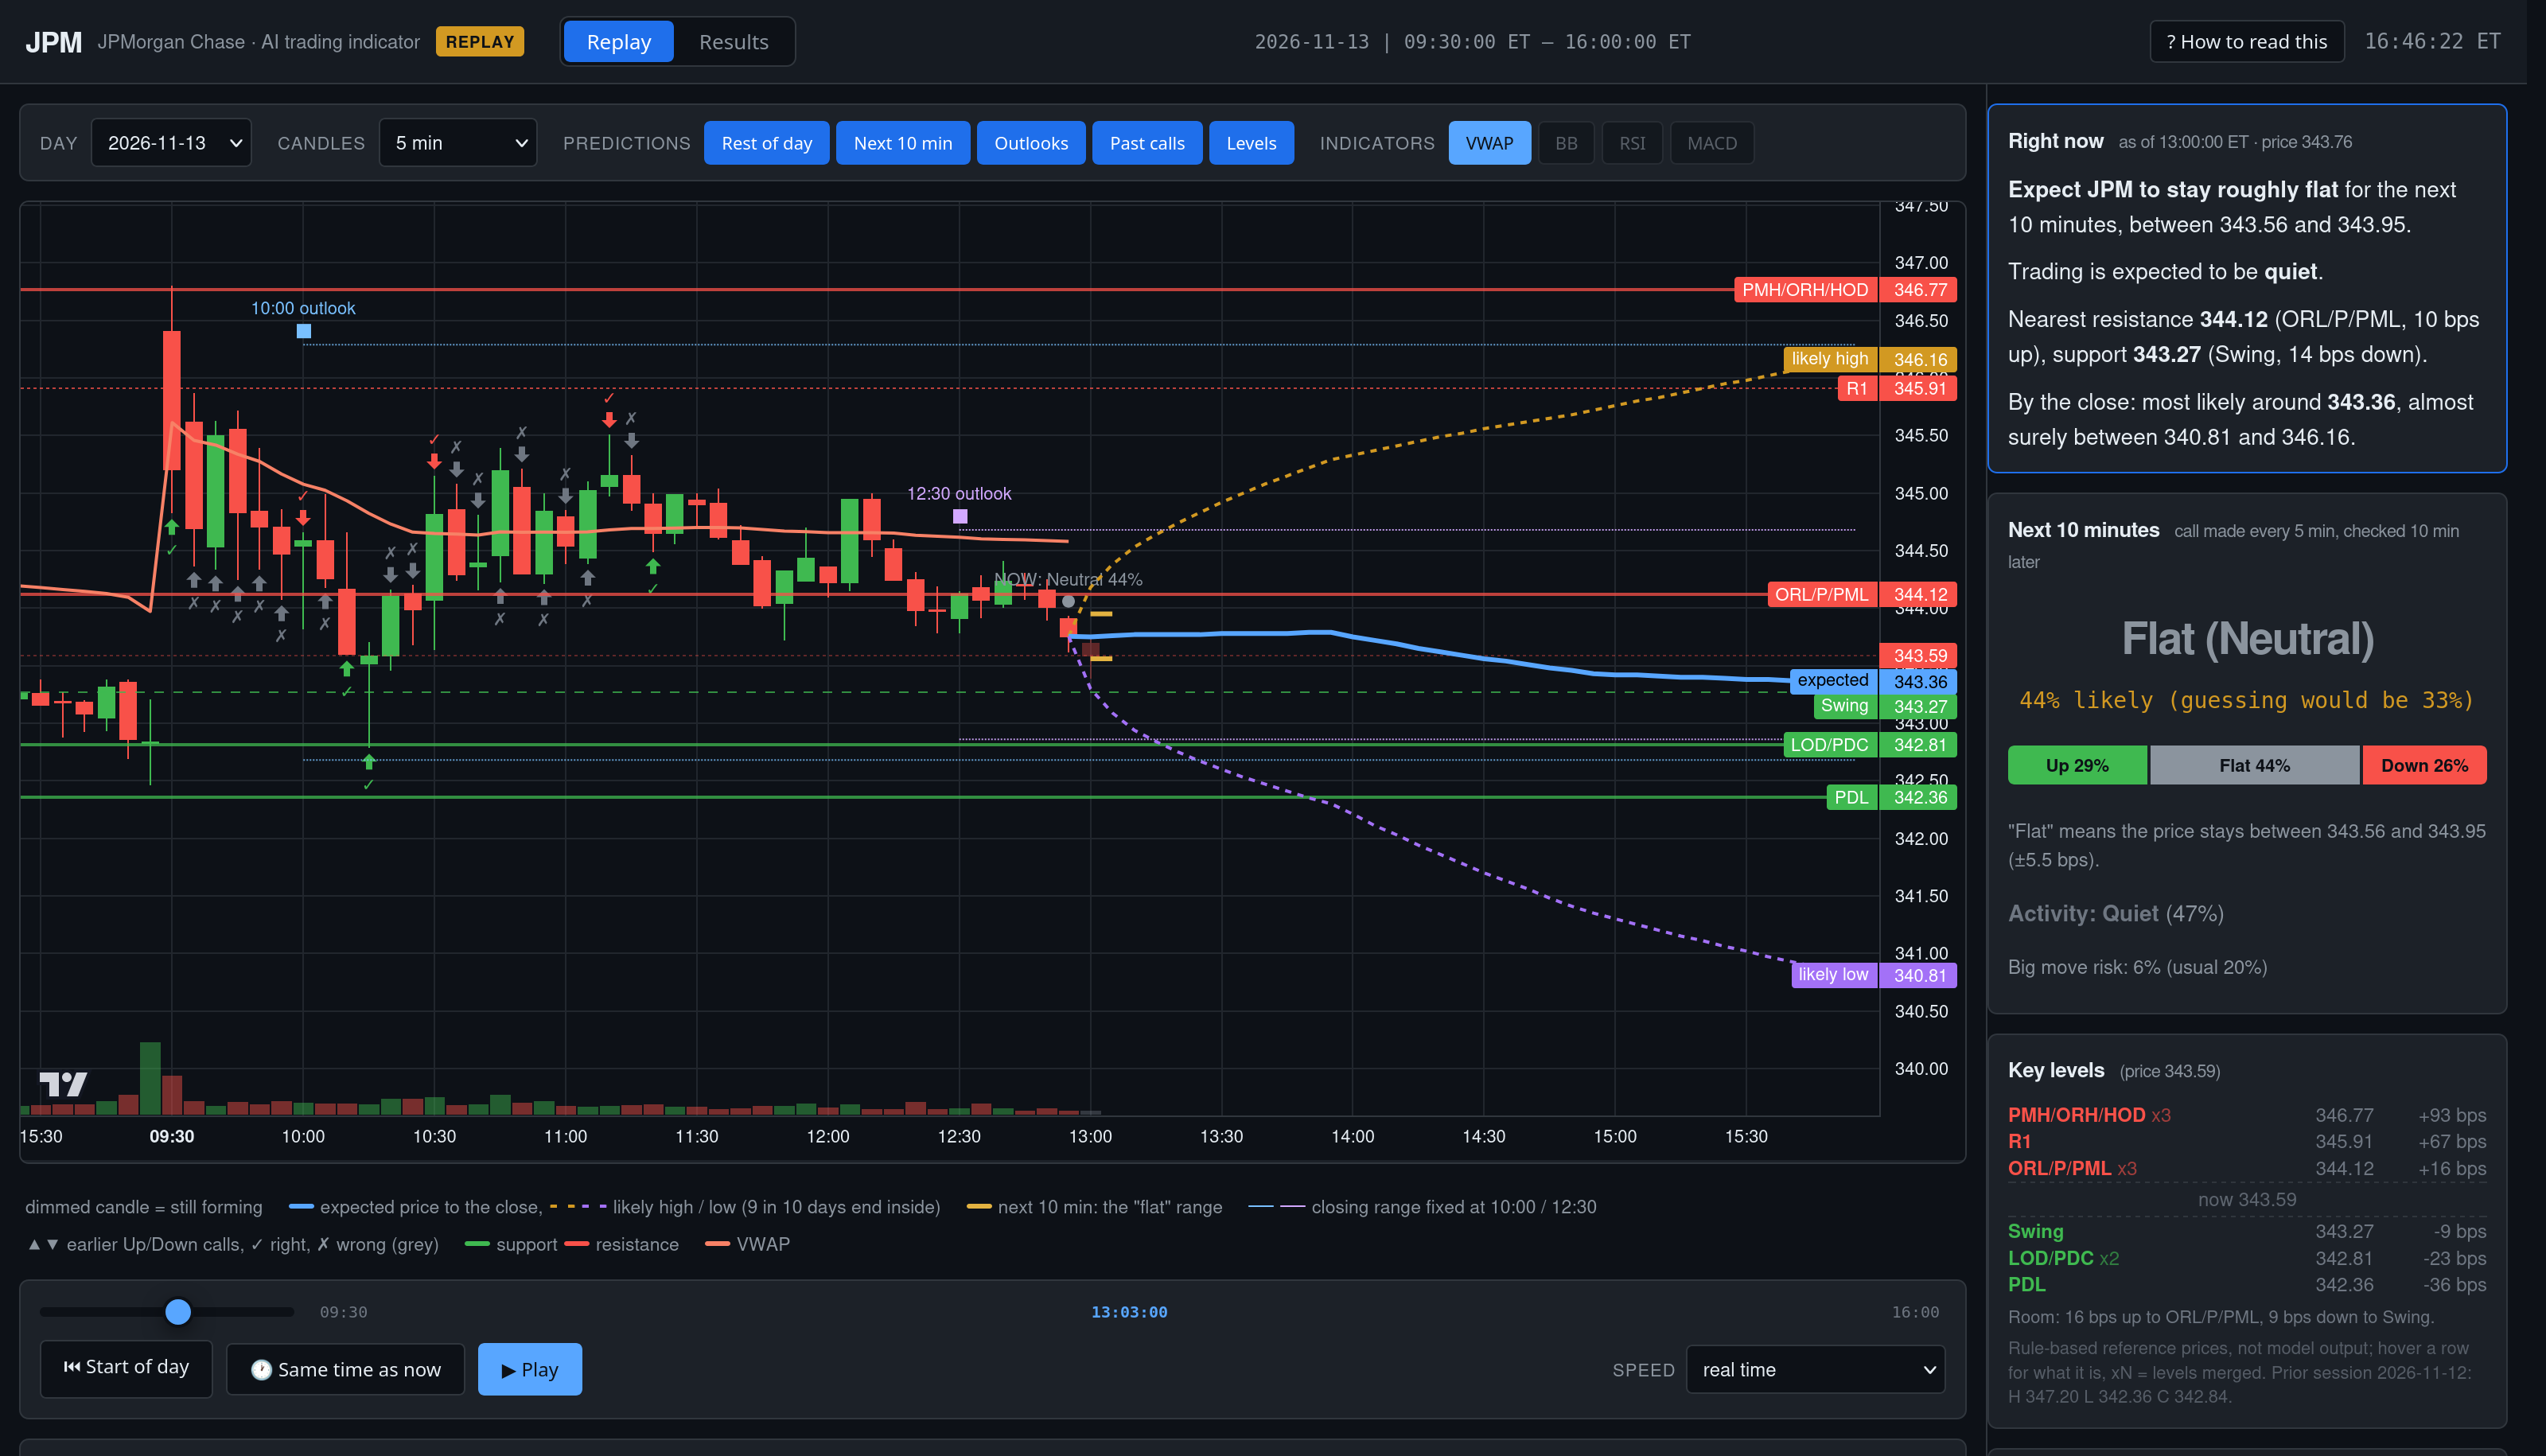
\includegraphics[width=0.8\textwidth]{ui_replay.png}
  \caption{Dashboard replaying 13 Nov 2026: candles, prediction layers, current call and the day's scorecard.}
  \label{fig:ui}
\end{figure*}

\subsection{Main result}
Test period: 2025-01-02 to 2026-10-27, 34,538 candles over 456 days. Validation was 2022--24 (56,843 candles).

\begin{table}[t]
\centering\small
\caption{3-class accuracy on the test period. Last column: share of test days where LightGBM beats that rule.}
\label{tab:main}
\setlength{\tabcolsep}{4pt}
\begin{tabular}{@{}l r r r@{}}
\toprule
Method & Acc. & Log-loss & Days won \\
\midrule
Always Flat & 32.8\,\% & -- & 80\,\% \\
Always Up & 34.1\,\% & -- & 70\,\% \\
RSI rule & 34.6\,\% & -- & 73\,\% \\
Persistence & 35.8\,\% & -- & 70\,\% \\
Log. regression & 39.7\,\% & 1.079 & -- \\
\textbf{LightGBM} & \textbf{40.7\,\%} & \textbf{1.065} & -- \\
LightGBM, 13 new days & 43.2\,\% & -- & -- \\
\bottomrule
\end{tabular}
\end{table}

LightGBM won on validation log-loss (1.066 vs 1.092 for logistic regression, 1.073 for the average of both) and stays
ahead on test (Table~\ref{tab:main}, Fig.~\ref{fig:acc}). A uniform guess has log-loss $\ln 3 = 1.099$. Probabilities
are well calibrated: ECE 0.6\,\%. On the 13 days after the cutoff (28 Oct -- 13 Nov 2026) accuracy was 43.2\,\% vs
36.8\,\% for persistence (per-day numbers in Appendix~\ref{app:holdout}).

\begin{figure*}[t]
  \centering
  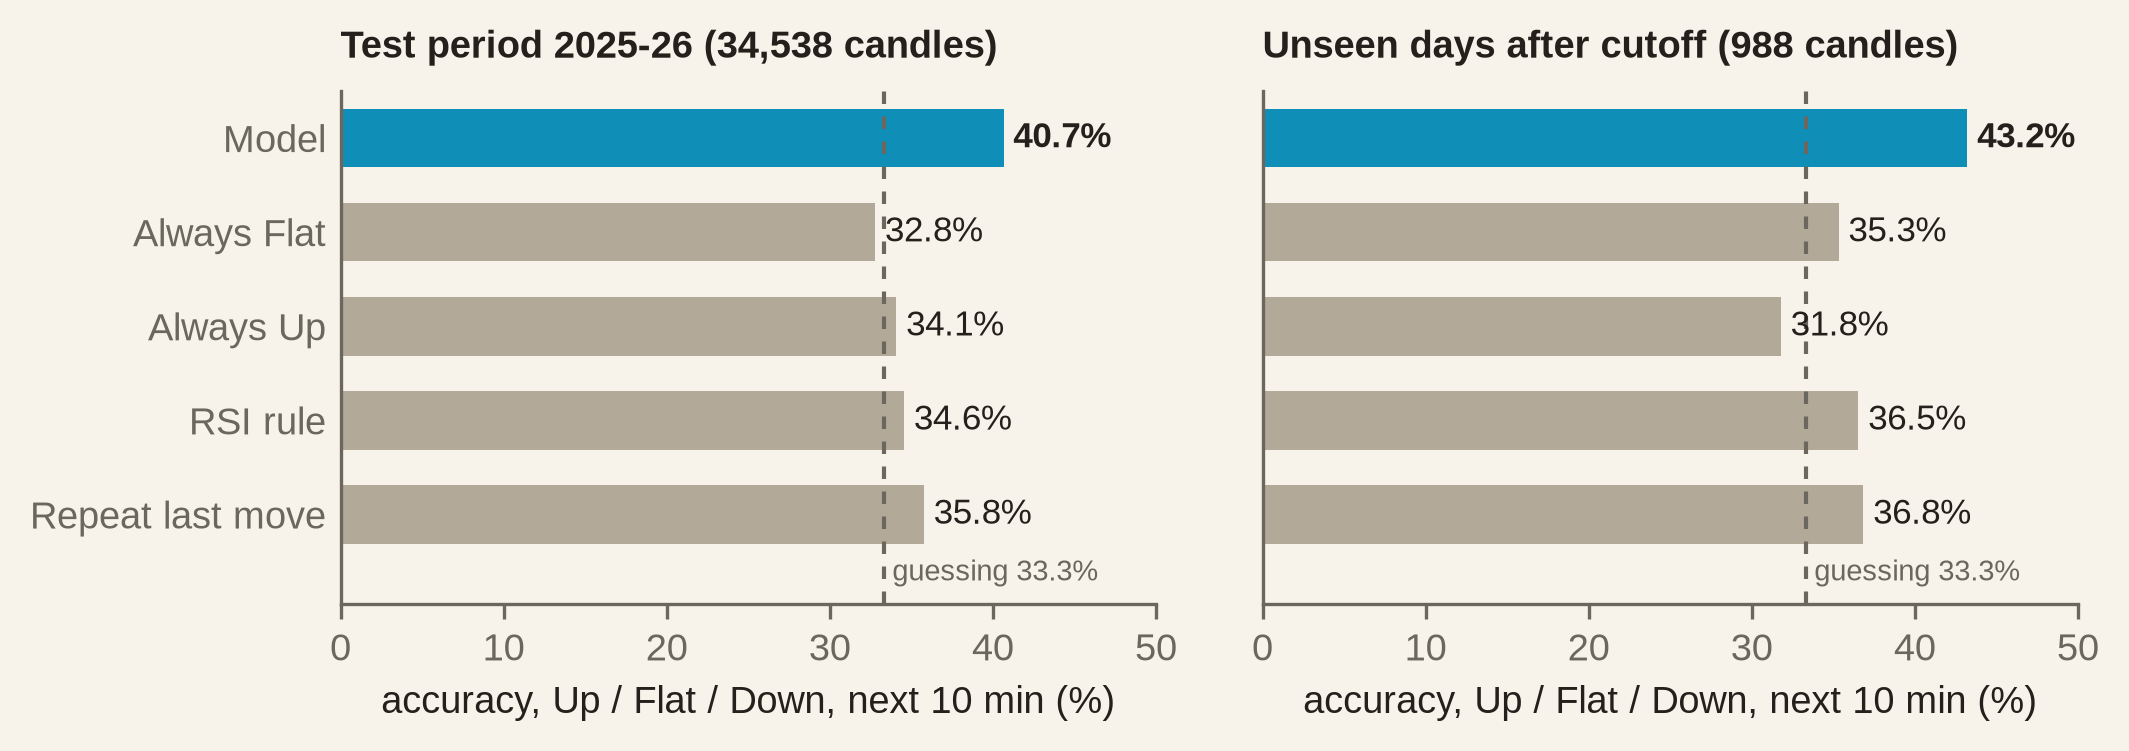
\includegraphics[width=0.85\textwidth]{fig_accuracy.png}
  \caption{Accuracy of our model (blue) vs simple rules; dashed line = random guess.}
  \label{fig:acc}
\end{figure*}

Single-day accuracy goes from 31.6\,\% (10th pct) to 50.0\,\% (90th pct), and the whole distribution sits to the
right of the best rule (Fig.~\ref{fig:daily}), so it is not a few lucky days. Feature importance
(Fig.~\ref{fig:imp}): volatility and range get 55\,\% of split gain, market and peers 13\,\%, order flow and news about
9\,\% each. So the model is mostly forecasting \emph{how much} the price will move.

\begin{figure}[t]
  \centering
  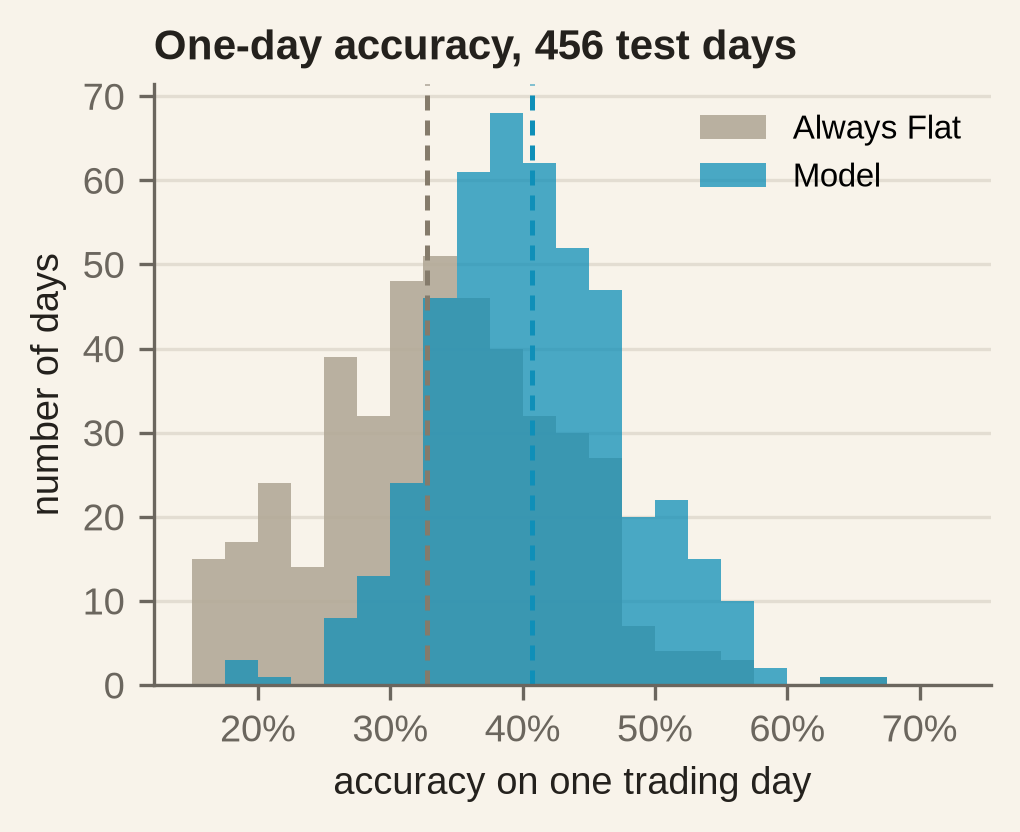
\includegraphics[width=0.85\columnwidth]{fig_daily.png}
  \caption{One-day accuracy over the 456 test days.}
  \label{fig:daily}
\end{figure}

\begin{figure}[t]
  \centering
  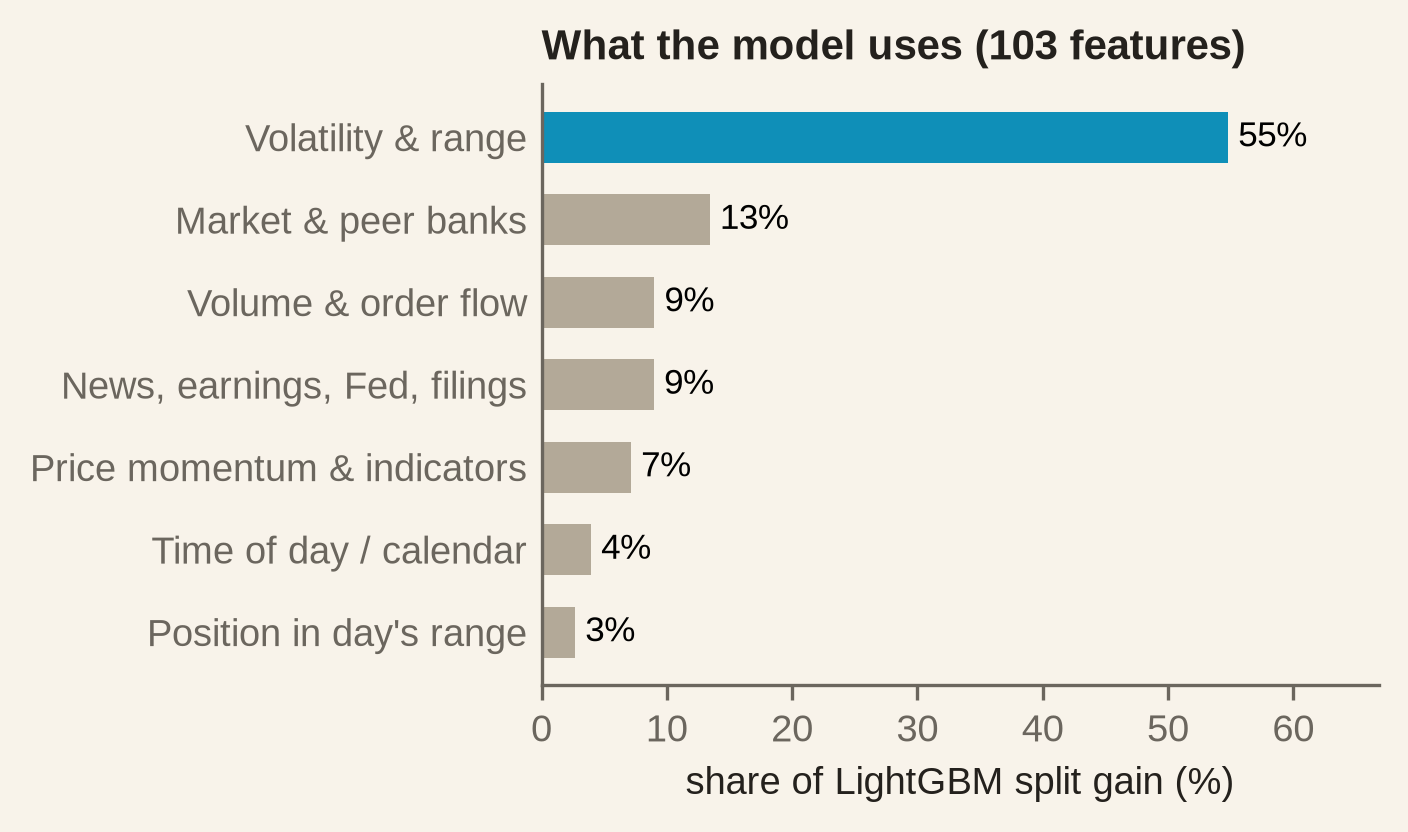
\includegraphics[width=\columnwidth]{fig_importance.png}
  \caption{Share of LightGBM split gain by feature family.}
  \label{fig:imp}
\end{figure}

\subsection{Other outputs}
\begin{table}[t]
\centering\small
\caption{Other outputs on the 2025--26 test period.}
\label{tab:other}
\footnotesize\setlength{\tabcolsep}{4pt}
\begin{tabularx}{\columnwidth}{@{}X r r@{}}
\toprule
Output & Ours & Baseline \\
\midrule
Activity (3 levels), acc. & 46.3\,\% & 40.2\,\% \\
Big-move warning, AUC & 0.785 & 0.5 \\
\ \ big moves in top-10\,\% risk & 57.7\,\% & 20.3\,\% \\
Next-minute direction, acc. & 51.8\,\% & 50.3\,\% \\
\ \ top-10\,\% most confident & 54.2\,\% & -- \\
Next-minute 90\,\% band cover & 90.4\,\% & 90\,\% \\
Rest-of-day 90/50\,\% band cover & 93.6/54.2\,\% & 90/50\,\% \\
Rest-of-day pinball (bps) & 14.0 & 15.1 \\
Up/Down calls, direction right & 49.6\,\% & 50\,\% \\
Per call after 2\,bps cost & $-2.21$\,bps & -- \\
\bottomrule
\end{tabularx}
\end{table}

Table~\ref{tab:other}. Activity and big-move outputs clearly beat their baselines and the bands hit their coverage
targets. On the unseen days the 10:00 forecast of the close put the actual close inside its 90\,\% band on 11 of 13
days (12:30 forecast: 13 of 13), but its lean up or down was right on only 7 of 13 (Fig.~\ref{fig:close}).

\begin{figure}[t]
  \centering
  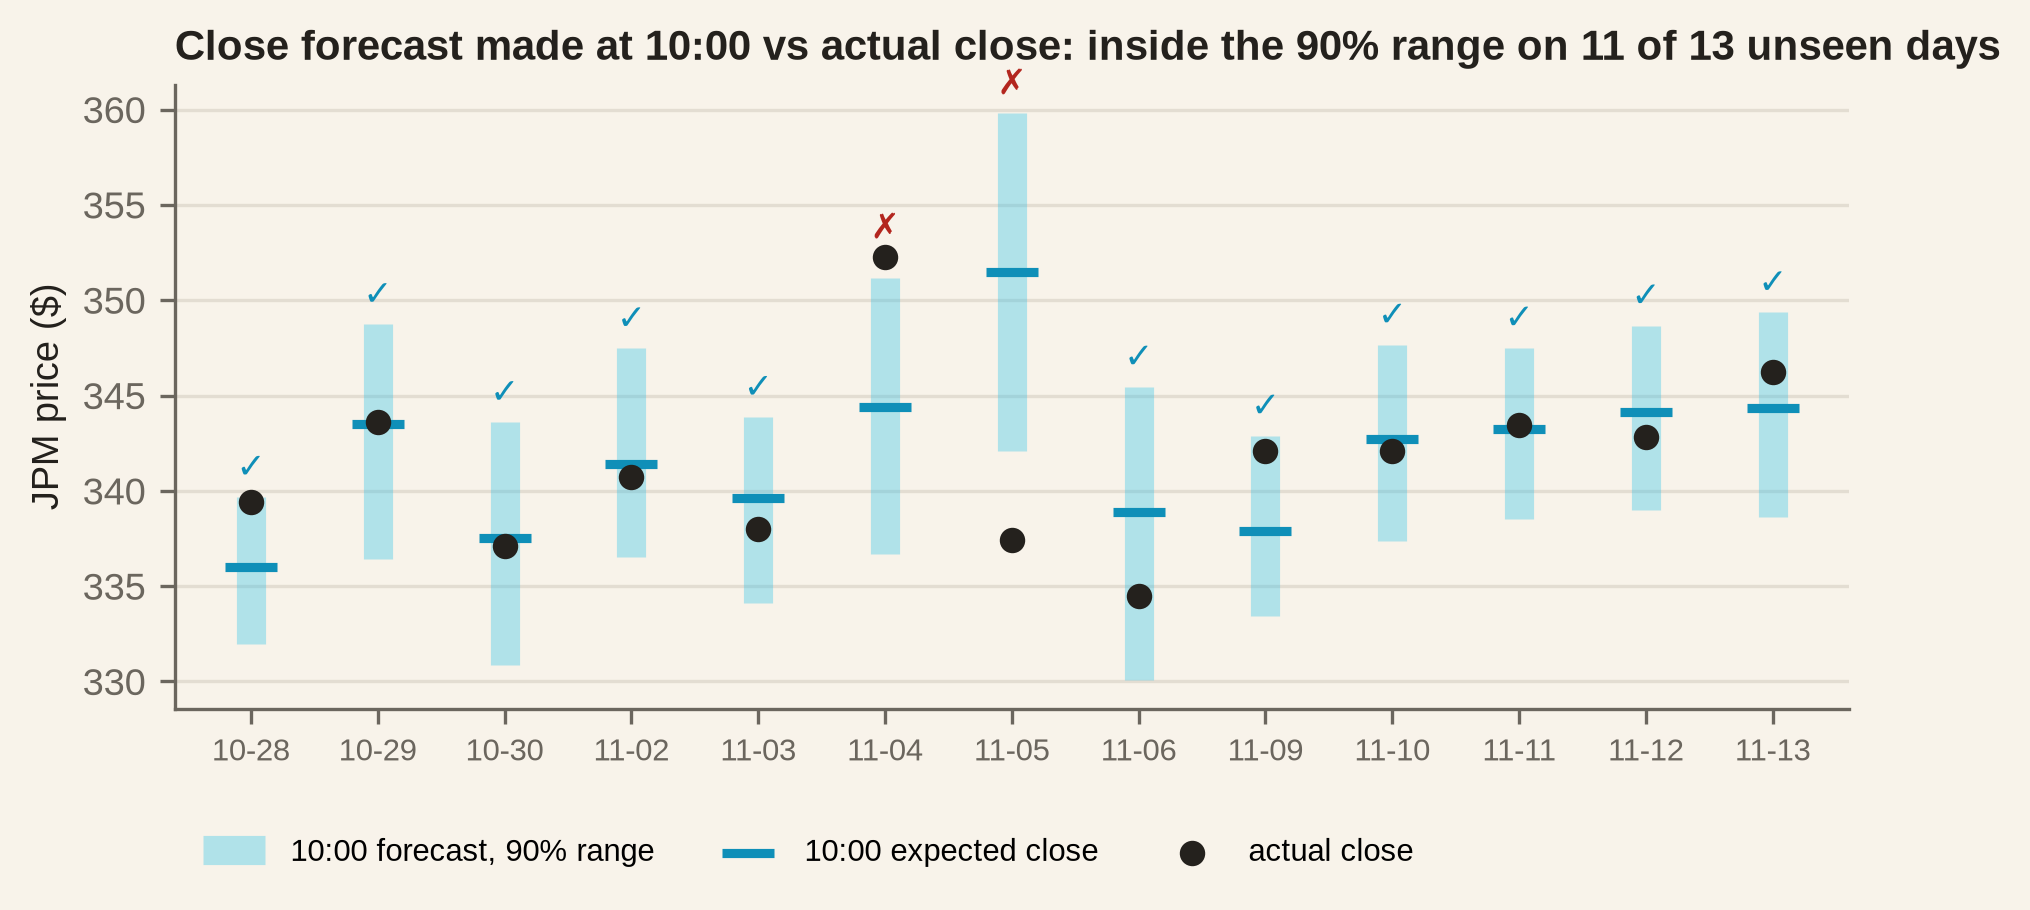
\includegraphics[width=\columnwidth]{fig_close.png}
  \caption{Close forecast at 10:00 (band, median) vs actual close, 13 unseen days.}
  \label{fig:close}
\end{figure}

\subsection{What did not work}
Before settling on 3 classes, we tried to predict plain Up vs Down for the next 30 minutes with ten model families, all
with the same features and walk-forward split (Table~\ref{tab:zoo}). None beat the 50.9\,\% base rate by more than
the $\pm$0.5-point 95\,\% interval. This matches the daily results in \cite{krauss2017,fischer2018} and is why we added
the Flat class and focused on move size.

\begin{table}[t]
\centering\small
\caption{30-min direction, test 2025--26 (32,530 rows, base rate 50.9\,\%).}
\label{tab:zoo}
\begin{tabular}{@{}l r r@{}}
\toprule
Model & Acc. & AUC \\
\midrule
Logistic regression & 50.6\,\% & 0.491 \\
LightGBM & 50.9\,\% & 0.509 \\
XGBoost & 50.8\,\% & 0.508 \\
CatBoost & 50.0\,\% & 0.499 \\
Extra-trees (clf / reg) & 50.1 / 50.9\,\% & 0.501 / 0.510 \\
MLP & 50.6\,\% & 0.491 \\
GRU \cite{cho2014} & 50.7\,\% & 0.498 \\
1-D CNN & 50.0\,\% & 0.490 \\
Transformer \cite{vaswani2017} & 50.6\,\% & 0.495 \\
Stacked ensemble & 51.1\,\% & 0.512 \\
\bottomrule
\end{tabular}
\end{table}

Other things that did not help: daily-horizon models (1 day / 1 week / 1 month, six banks pooled) got 51--54\,\%, below
always-up (53/57/60\,\%). FinBERT news scores, SEC filings, quarterly fundamentals, overnight/intraday splits, peer
lead-lag and pairs z-scores did not change this beyond noise. One next-day model scored 58.5\,\% on its most confident
25\,\% of days, but always-up got 56.5\,\% in the same period, the same slice got 49.2\,\% on validation, and it was
only 41 days, so we treat it as noise.

\subsection{Discussion}
\begin{itemize}
  \item The gain over baselines comes from the Flat class and the activity / big-move outputs. When the model calls
        Flat it is right 43.5\,\% of the time vs a 32.8\,\% base rate.
  \item Direction is not predictable here: 49.6\,\% on Up/Down calls and $-2.2$\,bps per call after costs. So the
        indicator is a risk/activity guide, not a buy/sell signal.
  \item Our numbers are lower than many published ones because of the strict checks, but they held up on the unseen
        days (43.2\,\% vs 40.7\,\% on test).
\end{itemize}

\subsection{Dashboard}
FastAPI + WebSocket server with a Lightweight Charts front end (Fig.~\ref{fig:ui}). It replays any session after the
training cutoff candle by candle, shows the call with its probabilities, activity, big-move risk, the price bands and
support/resistance lines, and grades each call once its 10 minutes are over. A results tab shows the test numbers and
per-day predicted vs actual.





% ================================================================
\section{Conclusion}
A LightGBM model on 103 causal features predicts the 10-min Up/Flat/Down class of JPM at 40.7\,\% on 2025--26 data it
never saw (best simple rule 35.8\,\%) and 43.2\,\% on 13 later days, with calibrated probabilities (ECE 0.6\,\%), a
useful big-move warning (AUC 0.785) and price bands that hit their coverage. It predicts how much the price will move,
not which way.

\textbf{Limitations.} No direction edge, so the calls cannot be traded profitably after costs. One stock and one
sector. Bars only, no order book, so order flow is approximated. News tone uses a general lexicon on headlines. The
unseen-day check is only 13 days.

\textbf{Future work.} Order-book data and real order-flow imbalance \cite{cont2014}; one model trained across many
banks; separate models for high- and low-volatility regimes; keep scoring the frozen model on new days.

% ================================================================
\begin{thebibliography}{99}
\footnotesize\setlength{\itemsep}{0pt}
\bibitem{fama1970} E.~F. Fama, ``Efficient capital markets: A review of theory and empirical work,'' \emph{J. Finance}, 25(2):383--417, 1970.
\bibitem{lo1988} A.~W. Lo, A.~C. MacKinlay, ``Stock market prices do not follow random walks,'' \emph{Rev. Financial Studies}, 1(1):41--66, 1988.
\bibitem{tetlock2007} P.~C. Tetlock, ``Giving content to investor sentiment: The role of media in the stock market,'' \emph{J. Finance}, 62(3):1139--1168, 2007.
\bibitem{brock1992} W.~Brock, J.~Lakonishok, B.~LeBaron, ``Simple technical trading rules and the stochastic properties of stock returns,'' \emph{J. Finance}, 47(5):1731--1764, 1992.
\bibitem{bailey2014} D.~H. Bailey, J.~M. Borwein, M.~L\'opez de Prado, Q.~J. Zhu, ``Pseudo-mathematics and financial charlatanism,'' \emph{Notices of the AMS}, 61(5):458--471, 2014.
\bibitem{gu2020} S.~Gu, B.~Kelly, D.~Xiu, ``Empirical asset pricing via machine learning,'' \emph{Rev. Financial Studies}, 33(5):2223--2273, 2020.
\bibitem{krauss2017} C.~Krauss, X.~A. Do, N.~Huck, ``Deep neural networks, gradient-boosted trees, random forests: Statistical arbitrage on the S\&P 500,'' \emph{EJOR}, 259(2):689--702, 2017.
\bibitem{fischer2018} T.~Fischer, C.~Krauss, ``Deep learning with long short-term memory networks for financial market predictions,'' \emph{EJOR}, 270(2):654--669, 2018.
\bibitem{chen2016} T.~Chen, C.~Guestrin, ``XGBoost: A scalable tree boosting system,'' \emph{KDD}, 2016.
\bibitem{ke2017} G.~Ke et al., ``LightGBM: A highly efficient gradient boosting decision tree,'' \emph{NeurIPS}, 2017.
\bibitem{prokhorenkova2018} L.~Prokhorenkova et al., ``CatBoost: Unbiased boosting with categorical features,'' \emph{NeurIPS}, 2018.
\bibitem{andersen1997} T.~G. Andersen, T.~Bollerslev, ``Intraday periodicity and volatility persistence in financial markets,'' \emph{J. Empirical Finance}, 4(2--3):115--158, 1997.
\bibitem{bollerslev1986} T.~Bollerslev, ``Generalized autoregressive conditional heteroskedasticity,'' \emph{J. Econometrics}, 31(3):307--327, 1986.
\bibitem{cont2014} R.~Cont, A.~Kukanov, S.~Stoikov, ``The price impact of order book events,'' \emph{J. Financial Econometrics}, 12(1):47--88, 2014.
\bibitem{lee1991} C.~M.~C. Lee, M.~J. Ready, ``Inferring trade direction from intraday data,'' \emph{J. Finance}, 46(2):733--746, 1991.
\bibitem{easley2012} D.~Easley, M.~L\'opez de Prado, M.~O'Hara, ``Flow toxicity and liquidity in a high-frequency world,'' \emph{Rev. Financial Studies}, 25(5):1457--1493, 2012.
\bibitem{hutto2014} C.~J. Hutto, E.~Gilbert, ``VADER: A parsimonious rule-based model for sentiment analysis of social media text,'' \emph{ICWSM}, 2014.
\bibitem{araci2019} D.~Araci, ``FinBERT: Financial sentiment analysis with pre-trained language models,'' arXiv:1908.10063, 2019.
\bibitem{guo2017} C.~Guo, G.~Pleiss, Y.~Sun, K.~Q. Weinberger, ``On calibration of modern neural networks,'' \emph{ICML}, 2017.
\bibitem{romano2019} Y.~Romano, E.~Patterson, E.~J. Cand\`es, ``Conformalized quantile regression,'' \emph{NeurIPS}, 2019.
\bibitem{lopezdeprado2018} M.~L\'opez de Prado, \emph{Advances in Financial Machine Learning}, Wiley, 2018.
\bibitem{cho2014} K.~Cho et al., ``Learning phrase representations using RNN encoder-decoder for statistical machine translation,'' \emph{EMNLP}, 2014.
\bibitem{vaswani2017} A.~Vaswani et al., ``Attention is all you need,'' \emph{NeurIPS}, 2017.
\end{thebibliography}

% ================================================================
\onecolumn
\appendix
\section{Code and how to run}
Code: \url{https://github.com/Sadashii/CS3103-PBL}
\begin{small}
\begin{verbatim}
uv sync                                                  # install dependencies
uv run python scripts/fetch_data.py                      # 1-min bars (Alpaca keys in .env)
uv run python scripts/train_cls3.py --cutoff 2026-10-27  # train + test
uv run python scripts/train_tick.py                      # next-minute model and price bands
uv run python scripts/holdout_eval.py                    # score the unseen days
uv run --with matplotlib python scripts/make_figures.py  # figures
uv run uvicorn server.app:app --port 8000                # dashboard
\end{verbatim}
\end{small}

\section{Results on the unseen days}
\label{app:holdout}
\begin{table}[H]
\centering\small
\caption{Per-day results after the training cutoff (76 labelled candles per day).}
\begin{tabular}{@{}l r r c c r r@{}}
\toprule
Day & Model acc. & Persistence & 10:00 lean right & Close in 10:00 band & Open (\$) & Close (\$) \\
\midrule
2026-10-28 & 35.5\,\% & 31.6\,\% & yes & yes & 337.38 & 339.39 \\
2026-10-29 & 63.2\,\% & 39.5\,\% & yes & yes & 344.51 & 343.59 \\
2026-10-30 & 32.9\,\% & 34.2\,\% & yes & yes & 345.29 & 337.09 \\
2026-11-02 & 42.1\,\% & 27.6\,\% & no  & yes & 340.95 & 340.75 \\
2026-11-03 & 34.2\,\% & 31.6\,\% & no  & yes & 340.00 & 338.01 \\
2026-11-04 & 31.6\,\% & 42.1\,\% & yes & no  & 346.00 & 352.25 \\
2026-11-05 & 50.0\,\% & 39.5\,\% & no  & no  & 358.64 & 337.41 \\
2026-11-06 & 40.8\,\% & 32.9\,\% & no  & yes & 333.15 & 334.49 \\
2026-11-09 & 46.1\,\% & 35.5\,\% & yes & yes & 339.00 & 342.07 \\
2026-11-10 & 47.4\,\% & 36.8\,\% & yes & yes & 343.96 & 342.11 \\
2026-11-11 & 44.7\,\% & 46.1\,\% & no  & yes & 342.89 & 343.44 \\
2026-11-12 & 47.4\,\% & 39.5\,\% & yes & yes & 345.75 & 342.84 \\
2026-11-13 & 46.1\,\% & 42.1\,\% & no  & yes & 346.41 & 346.22 \\
\midrule
All 13 days & 43.2\,\% & 36.8\,\% & 7 / 13 & 11 / 13 & & \\
\bottomrule
\end{tabular}
\end{table}

\end{document}
